\chapter{Progettazione}
\label{capitolo5}
\thispagestyle{empty}

\noindent Nei paragrafi successivi sono illustrate le fasi di implementazione del gestore di dati personali, motivando le scelte implementative e le eventuali differenze che si sono verificate rispetto a quanto detto in Analisi.

Per la realizzazione del gestore \`e stato utilizzato il linguaggio Java\cite{javalanguagespecs} \cite{java8api}.

Fra i principi generali seguiti in Progettazione troviamo l’inversione delle dipendenze, la separazione delle responsabilit\`a, il principio di sostituibilit\`a di Liskov e il gi\`a citato rasoio di Occam. Secondo il principio di inversione delle dipendenze, \`e necessario che le dipendenze presenti all’interno del codice non siano fra classi ma fra interfacce, in modo da evitare che la struttura possa risentire di cambiamenti che avvengono a basso livello. Il principio di separazione delle responsabilit\`a stabilisce che a ogni classe \`e attribuito un solo compito, da svolgere e completare interamente, ma mai pi\`u di uno: lo sviluppo di classi aventi pi\`u responsabilit\`a genera dipendenze non volute fra le classi, rendendo il codice fragile. Il principio di sostituibilit\`a di Liskov, infine, si applica ai casi di ereditariet\`a fra classi e ne regola il rapporto: ogni sottoclasse deve poter essere utilizzata al posto della classe base senza che sia evidenziata la differenza.

\section{Flusso del programma}
inserire grafico

\section{Accounting}
\label{sec:P-accounting}
\begin{figure} [h]
	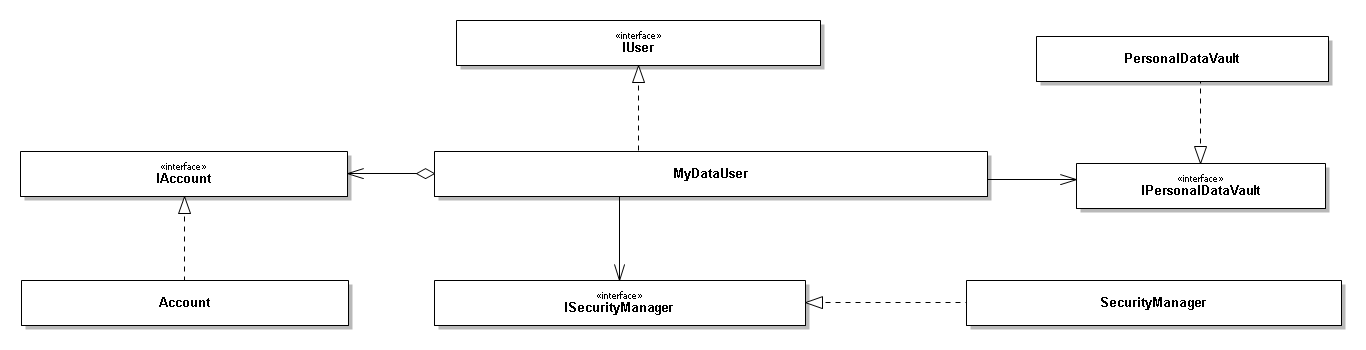
\includegraphics[width=\linewidth]{pictures/Accounting-closed.png}
	\caption{caption}
	\label{fig:Accounting-closed}
\end{figure}
Al centro \`e collocata la classe corrispondente all’utente \textit{MyData} che, confermando quanto detto in Analisi, \`e collegata agli account dei servizi e al \texttt{PersonalDataVault} dell’utente. Una novit\`a \`e invece rappresentata dalla coppia \texttt{ISecurityManager}, \texttt{SecurityManager} creata per soddisfare i requisiti di sicurezza relativi alla mutua autenticazione fra utente e servizio. Si \`e deciso di sviluppare separatamente questa classe per un principio di separazione delle responsabilit\`a e per consentire una estendibilit\`a pi\`u semplice in caso di sviluppi futuri.

\subsection{IUser, MyDataUser}
\begin{figure} [h]
	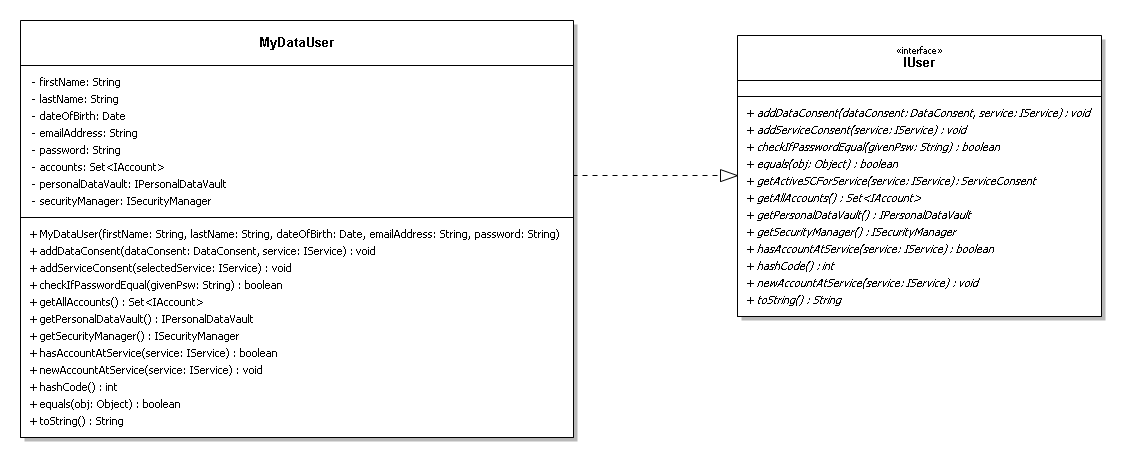
\includegraphics[width=\linewidth]{pictures/Accounting-MyDataUsr.png}
	\caption{caption}
	\label{fig:Accounting-MyDatUsr}
\end{figure}
Questa classe modella un generico utente dell’architettura \textit{MyData}. I field al suo interno sono un esempio delle caratteristiche che si \`e scelto di modellare e fra essi i pi\`u rilevanti sono indirizzo email e password in quanto permettono il login per utenti gi\`a registrati. L’indirizzo mail \`e stato adottato, inoltre, come identificatore unico di un utente all’interno di \textit{MyData} e questa caratteristica \`e stata implementata mediante l’override della funzione \texttt{equals(Object obj)}.

Si evidenzia inoltre la presenza di un \texttt{Set<IAccount> accounts} che realizza l’associazione fra un utente e gli account presso i servizi a cui si \`e registrato. La scelta di un \texttt{Set} permette di implementare il vincolo secondo cui ogni utente pu\`o avere un solo account presso un certo servizio ed \`e efficace anche perch\'e \`e superfluo mantenere un insieme ordinato di account.

Questa classe, inoltre, ha la funzione di interfacciare gli altri componenti del gestore, compresa la GUI, con gli account utente. A tal fine presenta i metodi \texttt{addServiceConsent} \texttt{(IService} \texttt{service)}, \texttt{addDataConsent} \texttt{(DataConsent} \texttt{dataConsent} \texttt{IService} \texttt{service)}, \texttt{hasAccountAtService} (\texttt{IService} \texttt{service)}.  La classe \texttt{Account}, infatti, \`e stata modellata con visibilit\`a package protected per impedire l’accesso a classi esterne al package \texttt{users}: di conseguenza, anche la creazione di nuovi account avviene attraverso questa classe, in particolare nella funzione \texttt{newAccountAtService} \texttt{(IService} \texttt{service)}. All’interno del metodo troviamo l’istanziazione di un nuovo account insieme ad una chiamata alla classe \texttt{ConsentManager} che realizza quanto anticipato al paragrafo \ref{sec:A-Consent} a pagina \pageref{sec:A-Consent}. In questo modo si ottiene un esempio di \textit{Service Linking} e l’esito di questa operazione viene concretizzato in un oggetto \texttt{ServiceConsent}. Si rimandano per\`o ulteriori dettagli a quanto evidenziato nella sezione \ref{sec:P-AutorizzazioniEConsent} a pagina \pageref{sec:P-AutorizzazioniEConsent}.

\subsection{IAccount, Account}
\begin{figure} [h]
	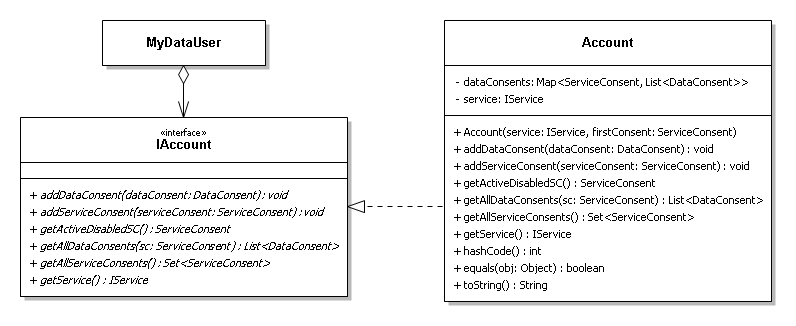
\includegraphics[width=\linewidth]{pictures/Accounting-Account.png}
	\caption{caption}
	\label{fig:Accounting-Account}
\end{figure}
La classe \texttt{Account} \`e abbastanza semplice, poich\'e si occupa semplicemente di implementare la logica di basso livello nelle operazioni di gestione degli account.

Fra queste vi sono i controlli sullo stato dei Consent memorizzati, la gestione dello storico di tutti i Consent emessi per quel servizio service, o ancora il matching fra i due tipi di Consent (\texttt{ServiceConsent}, \texttt{DataConsent}, dettagliati al paragrafo \ref{subsec:P-ServiceConsentDataConsent} a pagina \pageref{subsec:P-ServiceConsentDataConsent}).

La memorizzazione dei Consent all’interno della classe \`e stata ottenuta mediante l’utilizzo combinato delle strutture dati \texttt{Map<ServiceConsent,} \texttt{List<DataConsent>>}. Questa modalit\`a permette di esprimere diversi concetti a livello semantico. Come prima cosa, per i Consent sul flusso di dati si \`e scelto di utilizzare la classe base \texttt{DataConsent} invece che le sue due implementazioni, in modo da poterli memorizzare indiscriminatamente. Ci\`o verifica l’utilizzo del principio di sostituibilit\`a di Liskov. Inoltre, la scelta di una \texttt{List} come value all’interno di una mappa permette di descrivere un flusso di dati (all’interno dello stesso \texttt{ServiceConsent}) per il quale si sono rivelate necessare una molteplicit\`a di interazioni fra \textit{Source} e \textit{Sink}, ognuna delle quali modellata da un \texttt{DataConsent}.

Ad ogni istanza di \texttt{ServiceConsent} corrisponde quindi una \texttt{Collection} dei \texttt{DataConsent} emessi durante il periodo di validit\`a dello stesso, ed \`e possibile avere un unico \texttt{ServiceConsent} attivo in un determinato istante di tempo.

\section{SecurityManager}
\begin{figure} [h]
	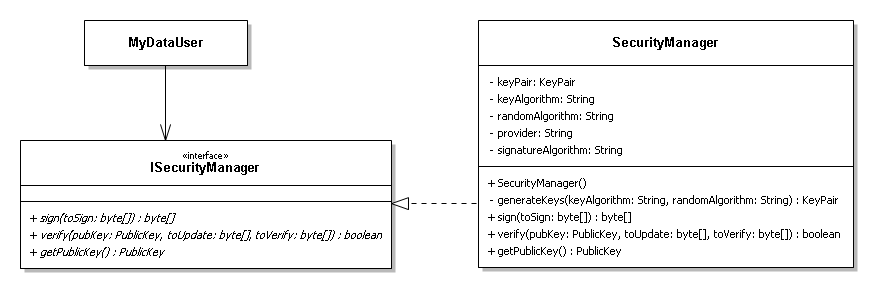
\includegraphics[width=\linewidth]{pictures/Accounting-SecurityManager.png}
	\caption{caption}
	\label{fig:Accounting-SecurityManager}
\end{figure}
Come anticipato nella sezione \ref{sec:P-accounting}, si \`e resa necessaria l'implementazione di una entit\`a che garantisse il rispetto di alcune politiche di sicurezza.

In particolare, in questa implementazione si \`e scelto di dare maggiore rilevanza all'aspetto di reciproca autenticazione fra utente e servizio, piuttosto che ad altre problematiche come ad esempio memorizzazione e trasmissione sicura dei dati. A tal fine, si \`e scelto di utilizzare alcuni componenti gi\`a pronti all'interno dell'infrastruttura Java, in particolare all'interno della Java Cryptography Architecture \cite{javacrypto}.

Per realizzare un protocollo di sfida e risposta, la classe \texttt{SecurityManager} contiene una coppia di chiavi \texttt{KeyPair}, insieme ad alcune costanti che rappresentano gli algoritmi ed il provider scelto per l'implementazione degli stessi.

L'interfaccia \texttt{ISecurityManager} ha la funzione di astrarre dalla particolare implementazione (ogni servizio potrebbe ad esempio preferire una implementazione specifica), e pertanto espone solamente i metodi di firma e verifica necessari al completamento dell'operazione di autenticazione.

\section{IMyData, MyData}
\begin{figure} [h]
	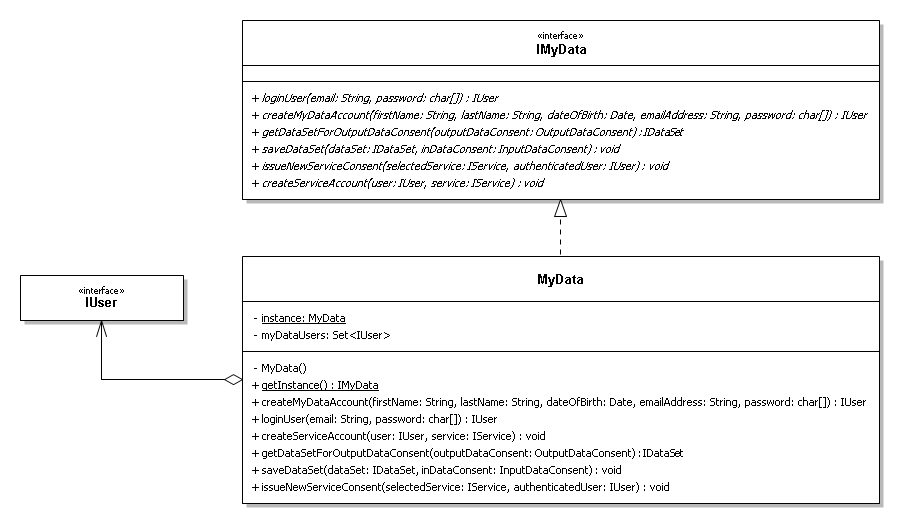
\includegraphics[width=\linewidth]{pictures/MyData.png}
	\caption{caption}
	\label{fig:Accounting-MyData}
\end{figure}
La classe \texttt{MyData} svolge all’interno del gestore di dati personali un importante ruolo di coordinazione fra le parti, poich\'e realizza al suo interno una parte dell’Operatore \textit{MyData}, secondo quanto specificato in \ref{sec:A-mydataop}. Essa \`e un punto di riferimento per l’interfaccia utente, alla quale fornisce i dati da elaborare e mostrare a video, e dalla quale riceve le richieste effettuate dall’utente.

Si occupa quindi come prima cosa di registrare e autenticare gli utenti (metodi \texttt{createMyDataAccount} e \texttt{loginUser}) in modo da impedire la creazione di duplicati. I controlli in questo senso vengono effettuati su un \texttt{HashSet<IUser>} contenuto all’interno della classe (si sfrutta la propriet\`a della struttura dati \texttt{Set} di non ammettere duplicati). La creazione di un nuovo account presso un determinato servizio viene gestita da questa classe, tramite invocazione dell’opportuno metodo esposto dall’interfaccia \texttt{IUser}, insieme alla richiesta di nuovi \texttt{ServiceConsent} in caso di utente gi\`a registrato.

In secondo luogo, ogni servizio che ha richiesto e ottenuto il permesso di accedere a uno specifico insieme di dati personali di un utente fa riferimento alla classe \texttt{MyData}, che si occupa di intercedere presso il Personal Data Vault per ottenere quanto richiesto. L’operazione si svolge sia per i dati in ingresso che per i dati in uscita dal Vault mediante i metodi \texttt{getDataSetForOutputDataConsent} \texttt{(OutputDataConsent} \texttt{outputDataConsent)} e \texttt{saveDataSet} \texttt{(IDataSet} \texttt{dataSet,} \texttt{InputDataConsent} \texttt{inDataConsent)}. In entrambi i casi, viene controllata la validit\`a del Consent emesso prima di effettuare la richiesta di dati personali.

Infine, si evidenzia la realizzazione della classe \texttt{MyData} come Singleton mediante l’utilizzo di un costruttore privato e di un campo \texttt{instance} di tipo \texttt{MyData}. Ci\`o assicura la presenza di un unico Operatore di questo tipo all’interno del programma.

\section{Autorizzazioni e Consent}
\label{sec:P-AutorizzazioniEConsent}
\begin{figure} [h]
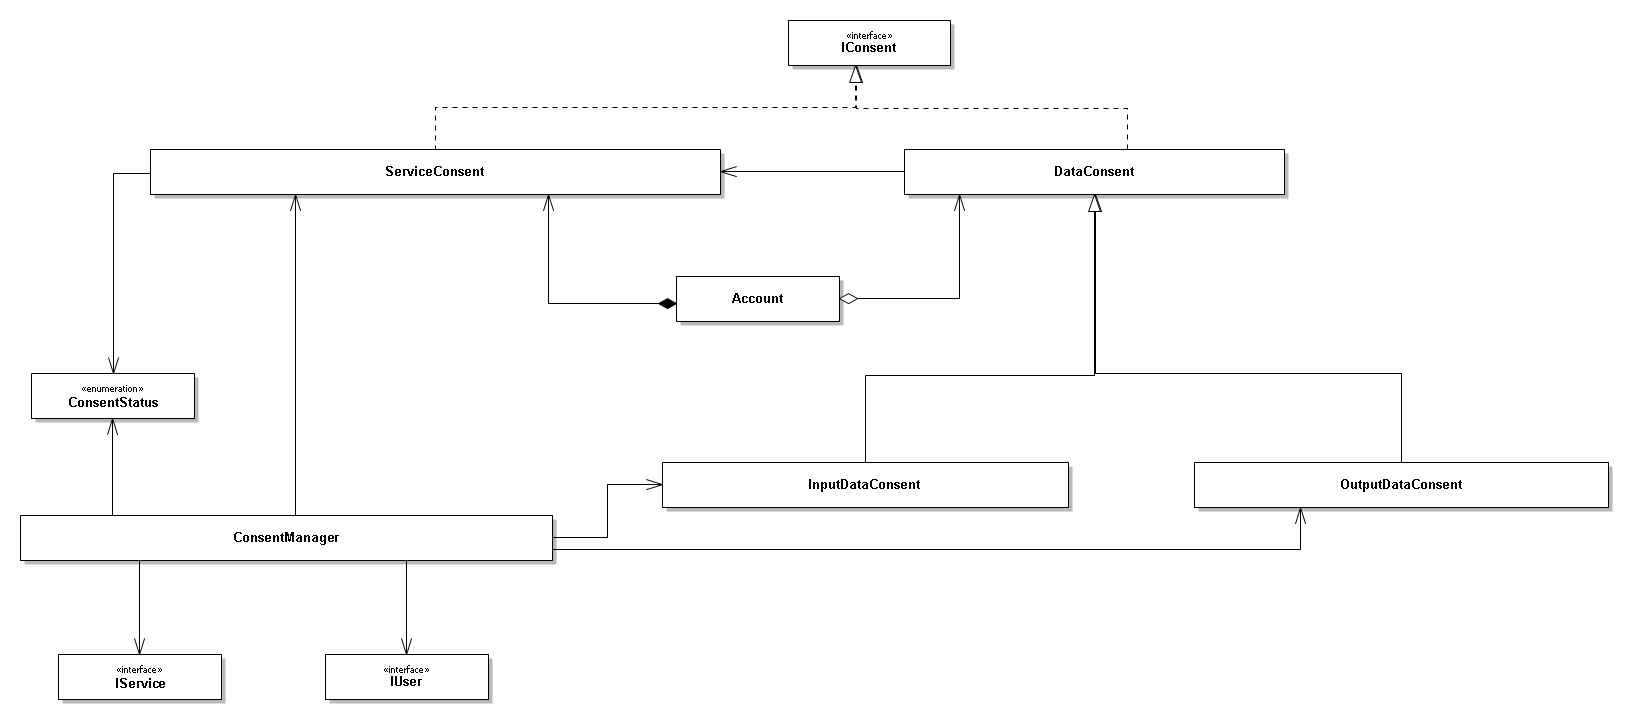
\includegraphics[width=\linewidth]{pictures/Auth-closed.png}
\caption{caption}
\label{fig:Auth-closed}
\end{figure}
All'interno dell'architettura realizzata per la gestione delle autorizzazioni e dei permessi \`e possibile individuare alcune entit\`a fondamentali: la classe \texttt{ConsentManager}, che realizza il gestore di permessi previsto nella sezione \ref{sec:A-mydataop}, e le due tipologie di permessi, anch’esse previste in fase di Analisi (sezione \ref{sec:A-Consent}).

\`E presente infine anche l’enumerativo \texttt{ConsentStatus}, attraverso il quale si rappresentano gli stati del rapporto fra un utente ed un servizio generici.


\subsection{ConsentManager, ConsentStatus}
\begin{figure} [h]
	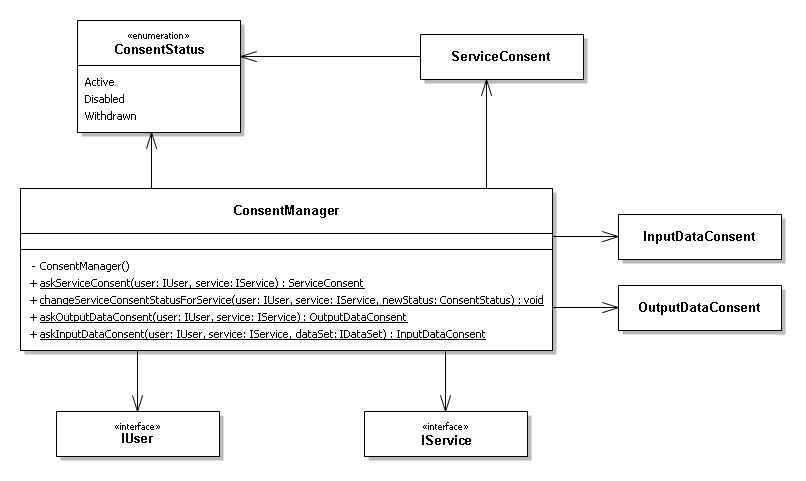
\includegraphics[width=\linewidth]{pictures/Auth-CM.png}
	\caption{caption}
	\label{fig:Auth-CM}
\end{figure}
La classe \texttt{ConsentManager} si occupa dell’erogazione, in caso di richiesta legittima, di vari tipi di permessi ai servizi che ne fanno richiesta. Poich\'e il suo scopo \`e quello di garantire il rispetto di un determinato protocollo di assegnazione dei permessi, essa \`e prima di tutto una classe implementativa e per questo motivo non \`e previsto alcun tipo di astrazione (ad esempio tramite interfaccia).

Si potrebbe considerare di rendere la classe \texttt{final}, per impedire estensioni o ridefinizioni del comportamento. Le motivazioni a supporto di questa scelta risiedono nella garanzia di una maggiore sicurezza. Tuttavia, nel complesso ci\`o avrebbe portato ad una eccessiva rigidit\`a del codice, impedendo aggiornamenti del protocollo anche in casi di legittima necessit\`a.

Per la sua implementazione, ho cercato di fare in modo che essa realizzasse un servizio il pi\`u possibile indipendente dal resto dell’architettura circostante. Pertanto, la classe \texttt{ConsentManager} non mantiene alcuno stato interno, presenta costruttore privato e non ha dipendenze rilevanti. Inoltre, poich\'e la procedura di verifica dei requisiti \`e costante e indipendente dai parametri di ingresso, ogni metodo \`e stato realizzato come \texttt{static}. 

I tipi di Consent erogati dalla classe \texttt{ConsentManager} sono \texttt{ServiceConsent} e le classi “figlie” \texttt{InputDataConsent}, \texttt{OutputDataConsent}, ognuno con un metodo dedicato. \`E presente anche la procedura \texttt{changeServiceConsentStatusForService} \texttt{(IUser} \texttt{user,} \texttt{IService} \texttt{service,} \texttt{ConsentStatus} \texttt{newStatus)}, che permette all’utente di cambiare lo stato del \texttt{ServiceConsent} correntemente attivo o disabilitato, secondo quanto previsto dalle specifiche di \textit{MyData} e successivamente in fase di Analisi (sezione \ref{sec:A-Consent}).


\subsection{ServiceConsent, DataConsent}
\label{subsec:P-ServiceConsentDataConsent}
\begin{figure} [h]
	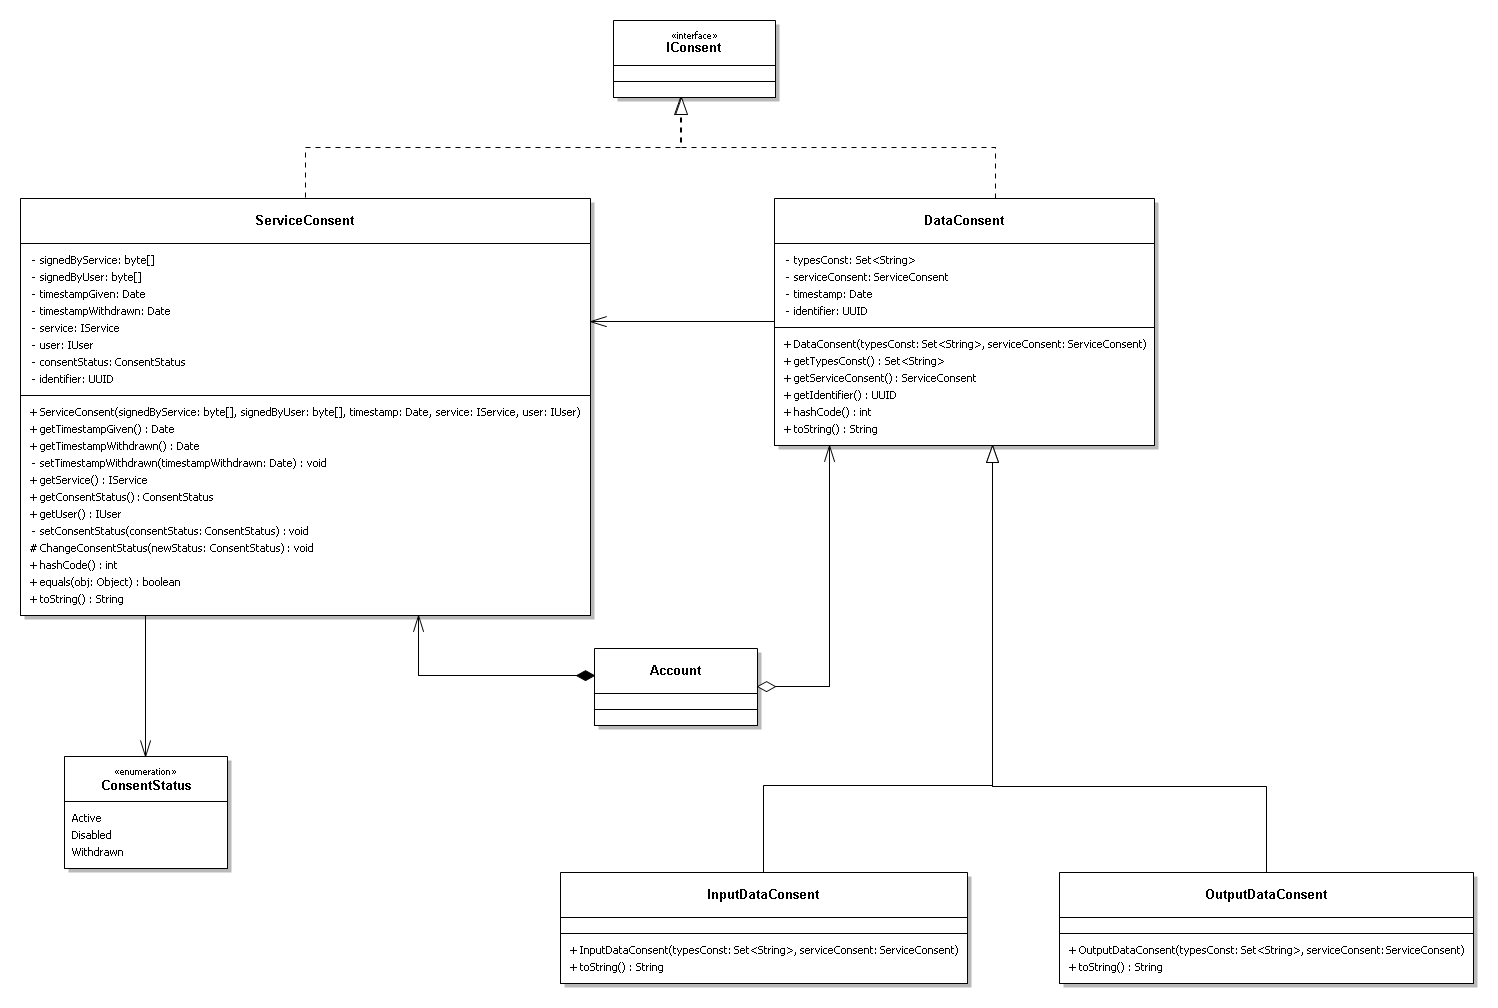
\includegraphics[width=\linewidth]{pictures/Auth-Consents.png}
	\caption{caption}
	\label{fig:Auth-Consents}
\end{figure}
https://docs.oracle.com/javase/8/docs/api/java/security/Permission.html

\section{PersonalDataVault}
\begin{figure} [h]
	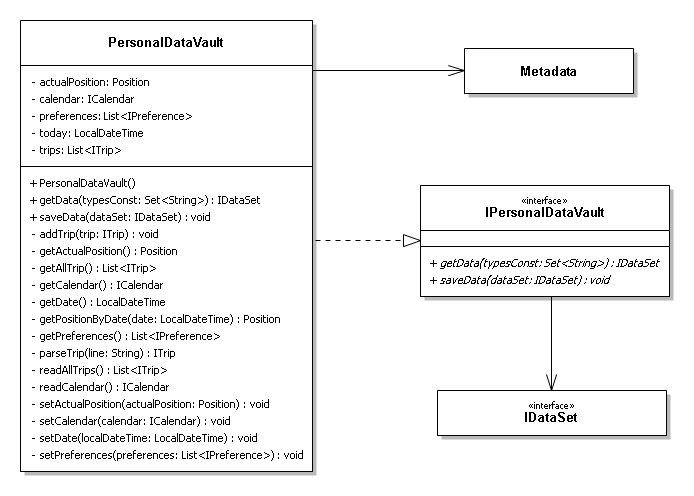
\includegraphics[width=\linewidth]{pictures/PersonalDataVault.png}
	\caption{caption}
	\label{fig:PersonalDataVault}
\end{figure}

\section{Metadata, DataSet}
\begin{figure} [h]
	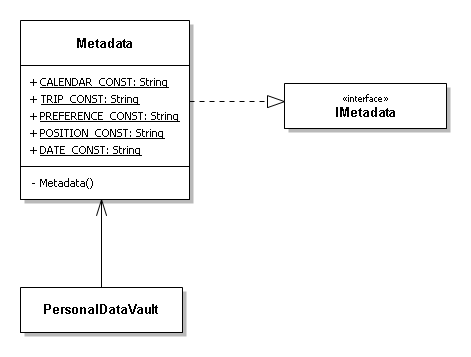
\includegraphics[width=\linewidth]{pictures/Metadata.png}
	\caption{caption}
	\label{fig:Metadata}
\end{figure}

\begin{figure} [h]
	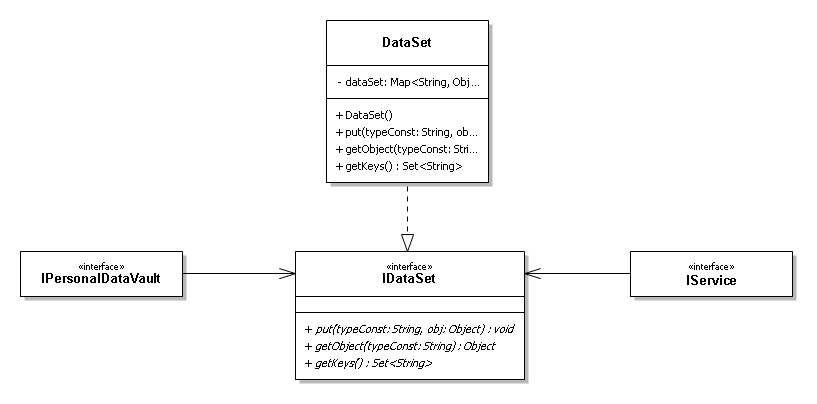
\includegraphics[width=\linewidth]{pictures/IDataSet.png}
	\caption{caption}
	\label{fig:IDataSet}
\end{figure}

\section{IService, AbstractService, MostLikelyNextTrip}
\begin{figure} [h]
	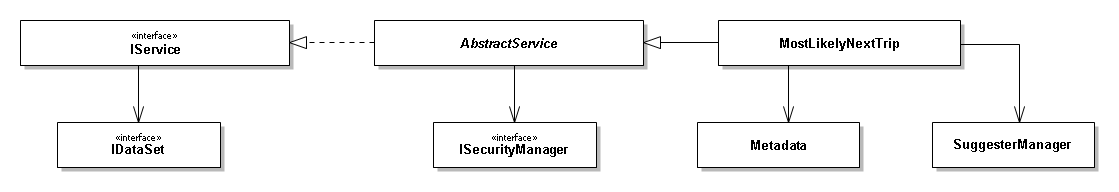
\includegraphics[width=\linewidth]{pictures/Services-closed.png}
	\caption{caption}
	\label{fig:Services-closed}
\end{figure}

\begin{figure} [h]
	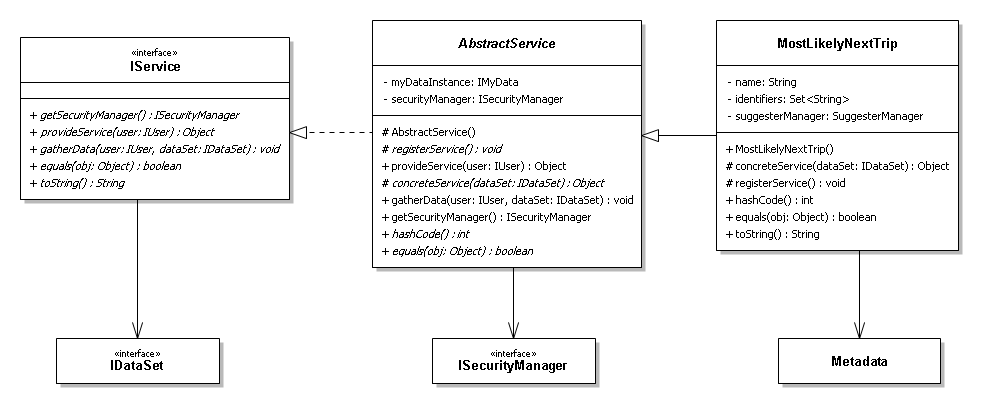
\includegraphics[width=\linewidth]{pictures/Services-open.png}
	\caption{caption}
	\label{fig:Services-open}
\end{figure}

\section{ServiceRegistry}
\begin{figure} [h]
	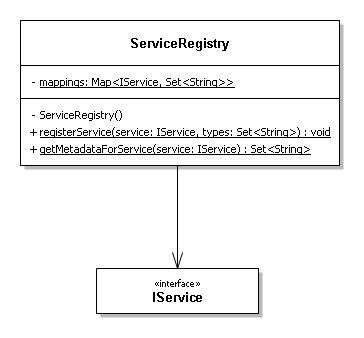
\includegraphics[width=\linewidth]{pictures/ServiceRegistry.png}
	\caption{caption}
	\label{fig:ServiceRegistry}
\end{figure}

\section{Uso delle eccezioni}